\chapter{Slovníkové techniky komprese}
\label{kapitolaSlovnikovaKomprese}
V předchozí kapitole jsme si představili kompresní techniky, které předpokládají zdroje generující posloupnosti nezávislých symbolů a snaží se vytvořit statistický model dat. Účinnost komprese pak závisí  na přesnosti modelu. Slovníkové techniky, které popíšu v~této kapitole, nepoužívají statistický model ani kódy s různou délkou kódových slov. Místo toho vyhledávají opakující se části textu, tzv. fráze, ty udržují ve slovníku a na výstup vypisují pouze odkaz na příslušné místo ve slovníku. Slovníkem zde může být jak část již zpracovaných dat, tak i vlastní struktura v paměti. Podobně jako u statistických modelů existují statické a adaptivní slovníky.

\section{Základy slovníkové komprese}
Základní princip a problematiku slovníkové komprese si můžeme představit na jednoduchém příkladu. Mějme text složený ze slov délky 5, kde jsou slova libovolně složena z arabských číslic a písmen A--F. Takováto abeceda má tedy 16 znaků. Pokud budeme předpokládat, že mají všechny znaky stejnou pravděpodobnost výskytu, budeme pro vytvoření binárního kódu potřebovat 4 bity na znak a 20 bitů k zakódování každého slova (těchto slov je $2^{20}$). Nyní vytvoříme statický slovník, který bude obsahovat 256 nejčastěji se vyskytujících slov.

Při kompresi budeme na výstup zapisovat jeden bit, charakterizující, zda je či není zpracovávané slovo obsaženo ve slovníku (např. 1 a 0), následovaný osmibitovým indexem slova (pokud je ve slovníku) nebo dvacetibitovým kódem slova (pokud ve slovníku není). To znamená, že pro slova ve slovníku potřebujeme pouze 9 bitů, zatímco pro slova, která ve slovníku nejsou, potřebujeme bitů 21.

Pro to, aby byl takovýto způsob komprese účinný, je rozhodující pravděpodobnost, že je zpracovávané slovo ve slovníku. To lze vyjádřit pomocí vzorce $R = Sp + T(1-p)$, kde $R$ je průměrný počet bitů na slovo, $S$ počet bitů pro slovo ve slovníku, $T$ počet bitů pro slovo mimo slovník a $p$ je pravděpodobnost, že je zpracovávané slovo ve slovníku. V našem případě musí být $R < 20$, což je splněno pro $p\geq 0,08\bar{3}$.

Pro pravděpodobnost $p$ blízkou číslu $0,08\bar{3}$ je účinnost komprese nízká a tedy nezajímavá. Pro vysokou účinnost potřebujeme pravděpodobnost $p$ co možná největší. Toho lze do\-sá\-hnout zvětšením slovníku, což s sebou nese vyšší paměťové nároky a časově náročnější prohledávání, nebo pečlivým výběrem slov ve slovníku.

\subsection{Typy slovníků}
V praxi jsou známy dva typy slovníků: statický a adaptivní. Podobně jako v případě statistických technik komprese (viz \ref{pravdepodobnostniModel}) je volba kompresního algoritmu se statickým slovníkem nejvhodnější, pokud známe dobře zdroj a komprimujeme zprávy výhradně tohoto zdroje. Proti tomu adaptivní slovník lze použít na neznámá data.

Většina kompresních algoritmů s adaptivním slovníkem je založena na pracích pánů Abrahama Lempela a Jacoba Ziva, kteří v letech 1977 a 1978 představili dva různé přístupy k~vytváření slovníku. Podle nich jsou vzniklé algoritmy označovány jako algoritmy rodiny LZ77, resp. LZ78.

\section{LZ77}
\label{lz77}
Princip tohoto algoritmu je založen na okně klouzajícím po zpracovávaných datech. Toto okno se dělí na dvě podokna (viz obrázek \ref{oknoLZ77}). V prvním je část ještě nezpracovaných dat. Ve druhém je pak část již zkomprimovaných dat, ve které jsou vyhledávány fráze a tedy funguje jako slovník. Velikost tohoto podokna je pevně daná jakožto kompromis mezi co největší velikostí, která zvyšuje pravděpodobnost nalezení fráze, a co nejmenší velikostí, která snižuje dobu vyhledávání fráze.

\begin{figure}[!htb]
\centering
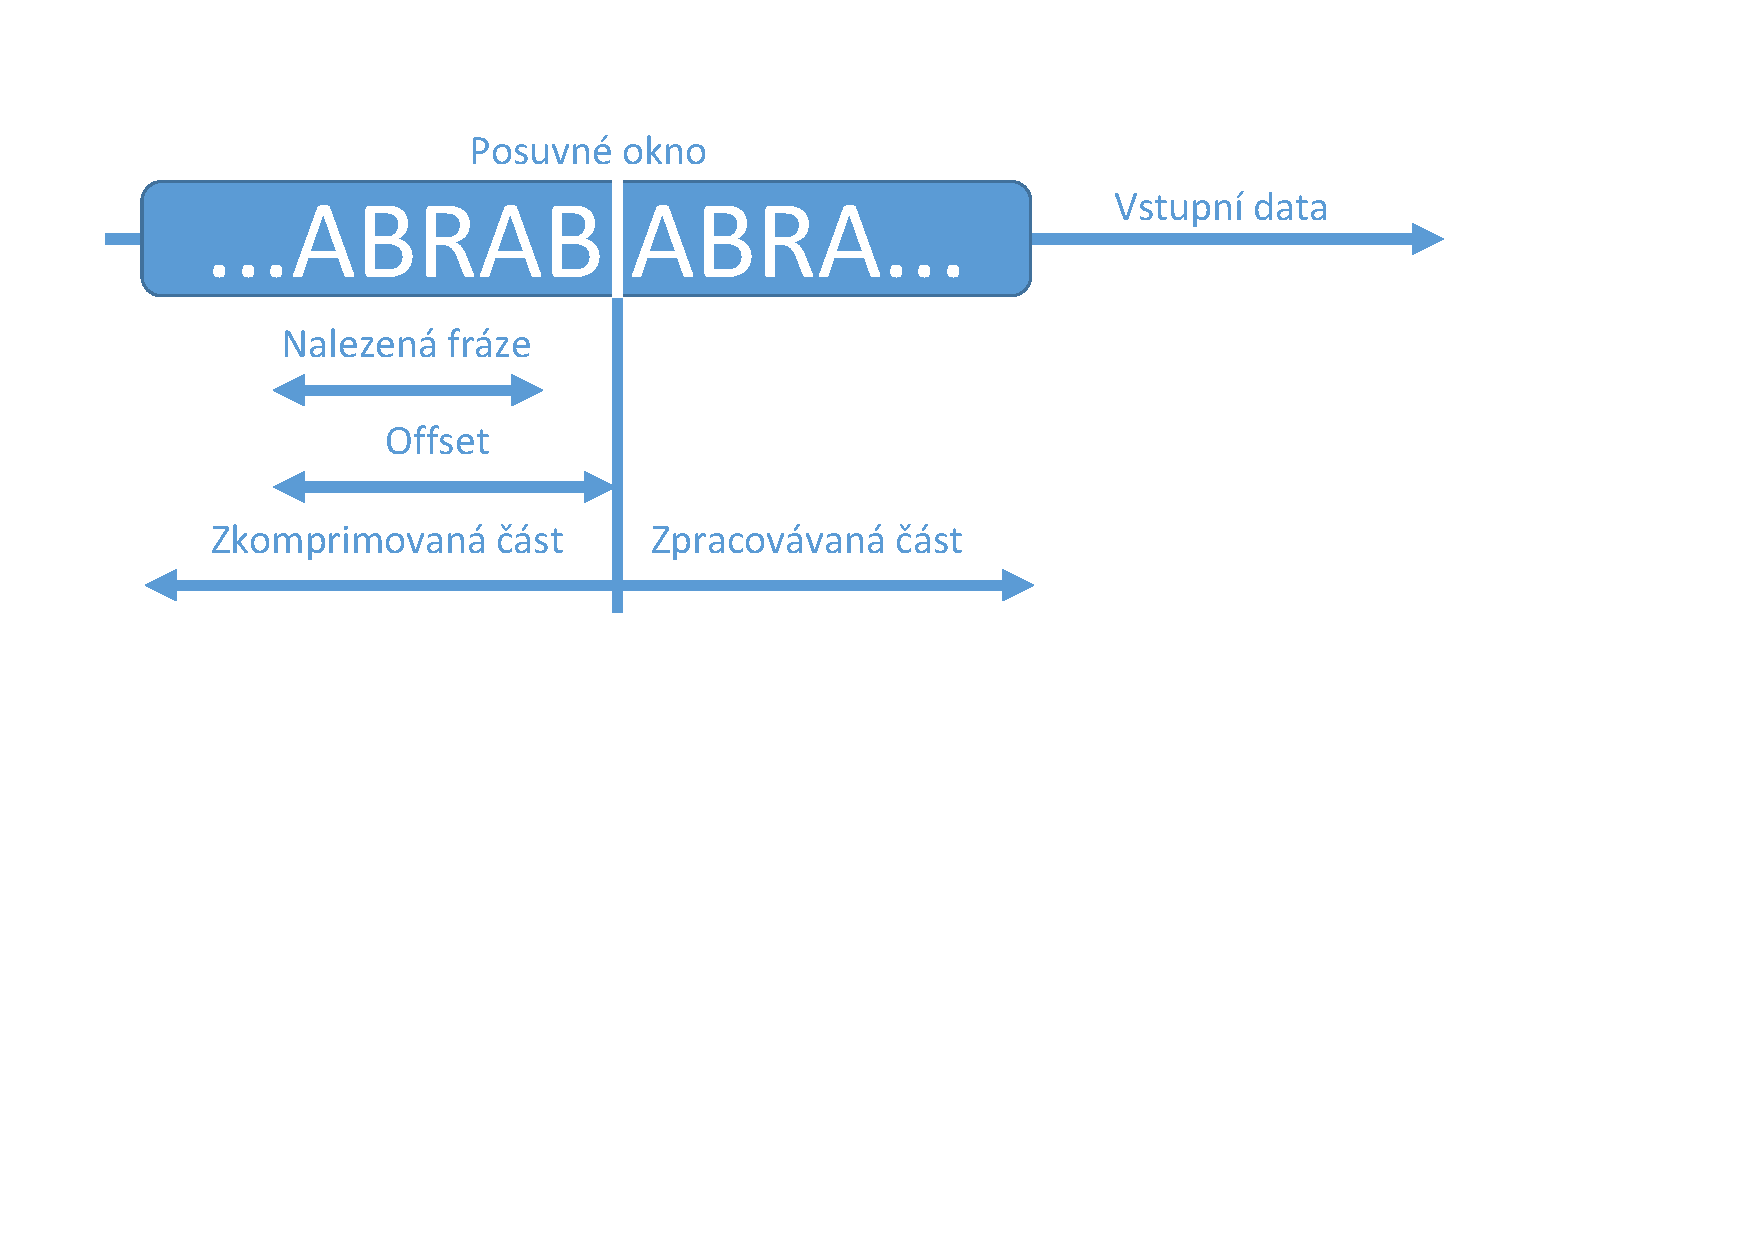
\includegraphics[trim=60 300 149 65, clip, angle=0, width=150mm]{oknoLZ77}
\caption{Schéma algoritmu LZ77, jenž využívá klouzavé okno}

\label{oknoLZ77}
\end{figure}

Tento algoritmus má velmi dobrý kompresní poměr pro data, ve kterých se shodné fráze vyskytují blízko sebe. To je dáno tím, že obsahem slovníku jsou poslední zpracovaná data, která se mění s posunem okna.

\subsection{Princip komprese}
V každém kroku kompresního algoritmu se v podokně zkomprimované části hledá nejdelší fráze. Znaky jsou procházeny zprava doleva až do shody prvního znaku fráze, kdy je zaznamenána délka fráze a vzdálenost fráze od pravého kraje podokna (offset), poté se pokračuje ve vyhledávání delší fráze dále vlevo. Nejdelší nalezená fráze je zakódována pomocí trojice (offset, délka fráze, následující znak (ve zpracovávaných datech)) a okno se posune o (délka fráze + 1) vpravo. Není-li nalezena shoda, je zakódován první znak ve zpracovávané části jako (0, 0, první znak). Tím je zaručeno, že se okno posune v každém kroku alespoň o jeden znak.

\subsection{Příklad komprese}
Zkusme zakódovat část textu začínajícího znaky ABRAKADABRAK s délkou podokna slovníku 7 znaků. V prvním kroku zakódujeme znak A, protože část slovníku je zatím prázdná, a posuneme okno o jeden znak doprava. Podobně zakódujeme i následující dva znaky B a R. Kódování jednotlivých znaků s offesetem 0 a délkou 0 je typickým projevem na začátku kompresního algoritmu, kdy je slovník ještě prázdný. V kroku 4 nalezneme frázi A délky 1 s offsetem 3 a posuneme okno o 2 znaky doprava. V dalším kroku úplně stejně zakódujeme další frázi A. V posledním kroku pak nalezneme frázi ABRA délky 4 s~offsetem 7, kterou zakódujeme jako (7,4,K). Celý postup je zobrazen v tabulce \ref{LZ77tabulka}.

\begin{table}[!htb]
\centering
\begin{tabular}{|c|c|c|c|}
\hline
Krok & Text & Fráze & Kódování\\
\hline
1 & \boxed{\mathrm{\textcolor{white}{ABRAKAD}}}\boxed{\mathrm{ABRAK}}ADABRAK\ldots & & (0,0,A)\\
&&&\\
2 & \textcolor{white}{A}\boxed{\mathrm{\textcolor{white}{WWWAK}A}}\boxed{\mathrm{BRAKA}}DABRAK\ldots & & (0,0,B)\\
&&&\\
3 & \textcolor{white}{AA}\boxed{\mathrm{\textcolor{white}{WARAK}AB}}\boxed{\mathrm{RAKAD}}ABRAK\ldots & & (0,0,R)\\
&&&\\
4 & \textcolor{white}{AAA}\boxed{\mathrm{\textcolor{white}{WAAA}ABR}}\boxed{\mathrm{AKADA}}BRAK\ldots & A & (3,1,K)\\
&&&\\
5 & \textcolor{white}{AAAAA}\boxed{\mathrm{\textcolor{white}{WA}ABRAK}}\boxed{\mathrm{ADABR}}AK\ldots & A & (2,1,D)\\
&&&\\
6 & \textcolor{white}{AAAAAAA}\boxed{\mathrm{ABRAKAD}}\boxed{\mathrm{ABRAK}}\ldots & ABRA & (7,4,K)\\
\hline
\end{tabular}
\caption{Kódování textu pomocí algoritmu LZ77}
\label{LZ77tabulka}
\end{table}

\subsection{Princip dekomprese}
Postup dekomprese je mnohem jednodušší a rychlejší než kompresní algoritmus. V paměti si udržuje pouze data slovníku, ve kterém jednoduše vyhledává fráze dle postupně de\-kó\-do\-va\-ných trojic. Offset a délka fráze určují frázi jednoznačně a není tedy nutné prohledávat celý slovník. LZ77 je tedy asymetrický kompresní algoritmus.

\subsection{Variace algoritmu LZ77}
Vylepšených verzí algoritmu LZ77 vzniklo několik a lze je rozdělit do skupin dle způsobu zlepšení. První skupina je zaměřena na efektivní kódování výstupu, tj. výše popsaných trojic, pomocí kódu s proměnlivou délkou slov. Reprezentantem takového kódóvání jsou semiadaptivní a adaptivní Huffmanovo kódování (viz \ref{huffmanovoKodovani} a \ref{adaptivniHuffman}). Další skupina pracuje s~proměnlivou velikostí klouzavého okna, což pro případ jeho zvětšení nese požadavek na implementaci efektivnějších vyhledávacích algoritmů.

Velmi známá verze je algoritmus LZSS, který odstraňuje neefektivní chování původního algoritmu, kdy je v jednom kroku kódován i následující znak, kterým může začínat fráze existující ve slovníku. Místo toho jsou nalezené fráze kódovány pomocí trojice (příznak, offset, délka fráze) a samotné znaky, které nejsou nalezeny ve slovníku, pomocí dvojice (příznak, znak).

\section{LZ78}
Algoritmus je založen na vyhledávání opakujících se frází ve vlastní paměťové struktuře. Tento slovník je na začátku procesu prázdný a postupně jsou do něho při zpracování na indexované pozice vkládány jednotlivé fráze. Jednoduché schéma je zobrazeno na obrázku \ref{slovnikLZ78}. Podobně jako v případě LZ77 je velikost slovníku dána kompromisem mezi počtem uložených frází a rychlostí vyhledávání.

V případě, že je slovník zcela naplněn, algoritmus LZ78 neříká přesně, co v takové situaci udělat. Existuje ale několik možností, které se v praxi používají a jsou vhodné pro různé případy.

\begin{itemize}
\item Dále využívat slovník jako statický. To je vhodné v případě, že se stejné fráze opakují v celé šířce dat.
\item Slovník úplně vymazat a začít ho plnit znovu. Takový přístup lze s výhodou aplikovat na data, ve kterých lze nalézt velké ucelené bloky, ve kterých se opakují různé fráze. Zároveň tento přístup připomíná princip algoritmu LZ77, kdy je jako slovník použita část blízkých předcházejících dat.
\item Ze slovníku mazat fráze s nízkým výskytem. Takto adaptivní slovník by byl vhodný univerzálně, nicméně není znám algoritmus, který by dokázal určit, kolik a kterých frází má být smazáno.
\end{itemize}

\begin{figure}[!htb]
\centering
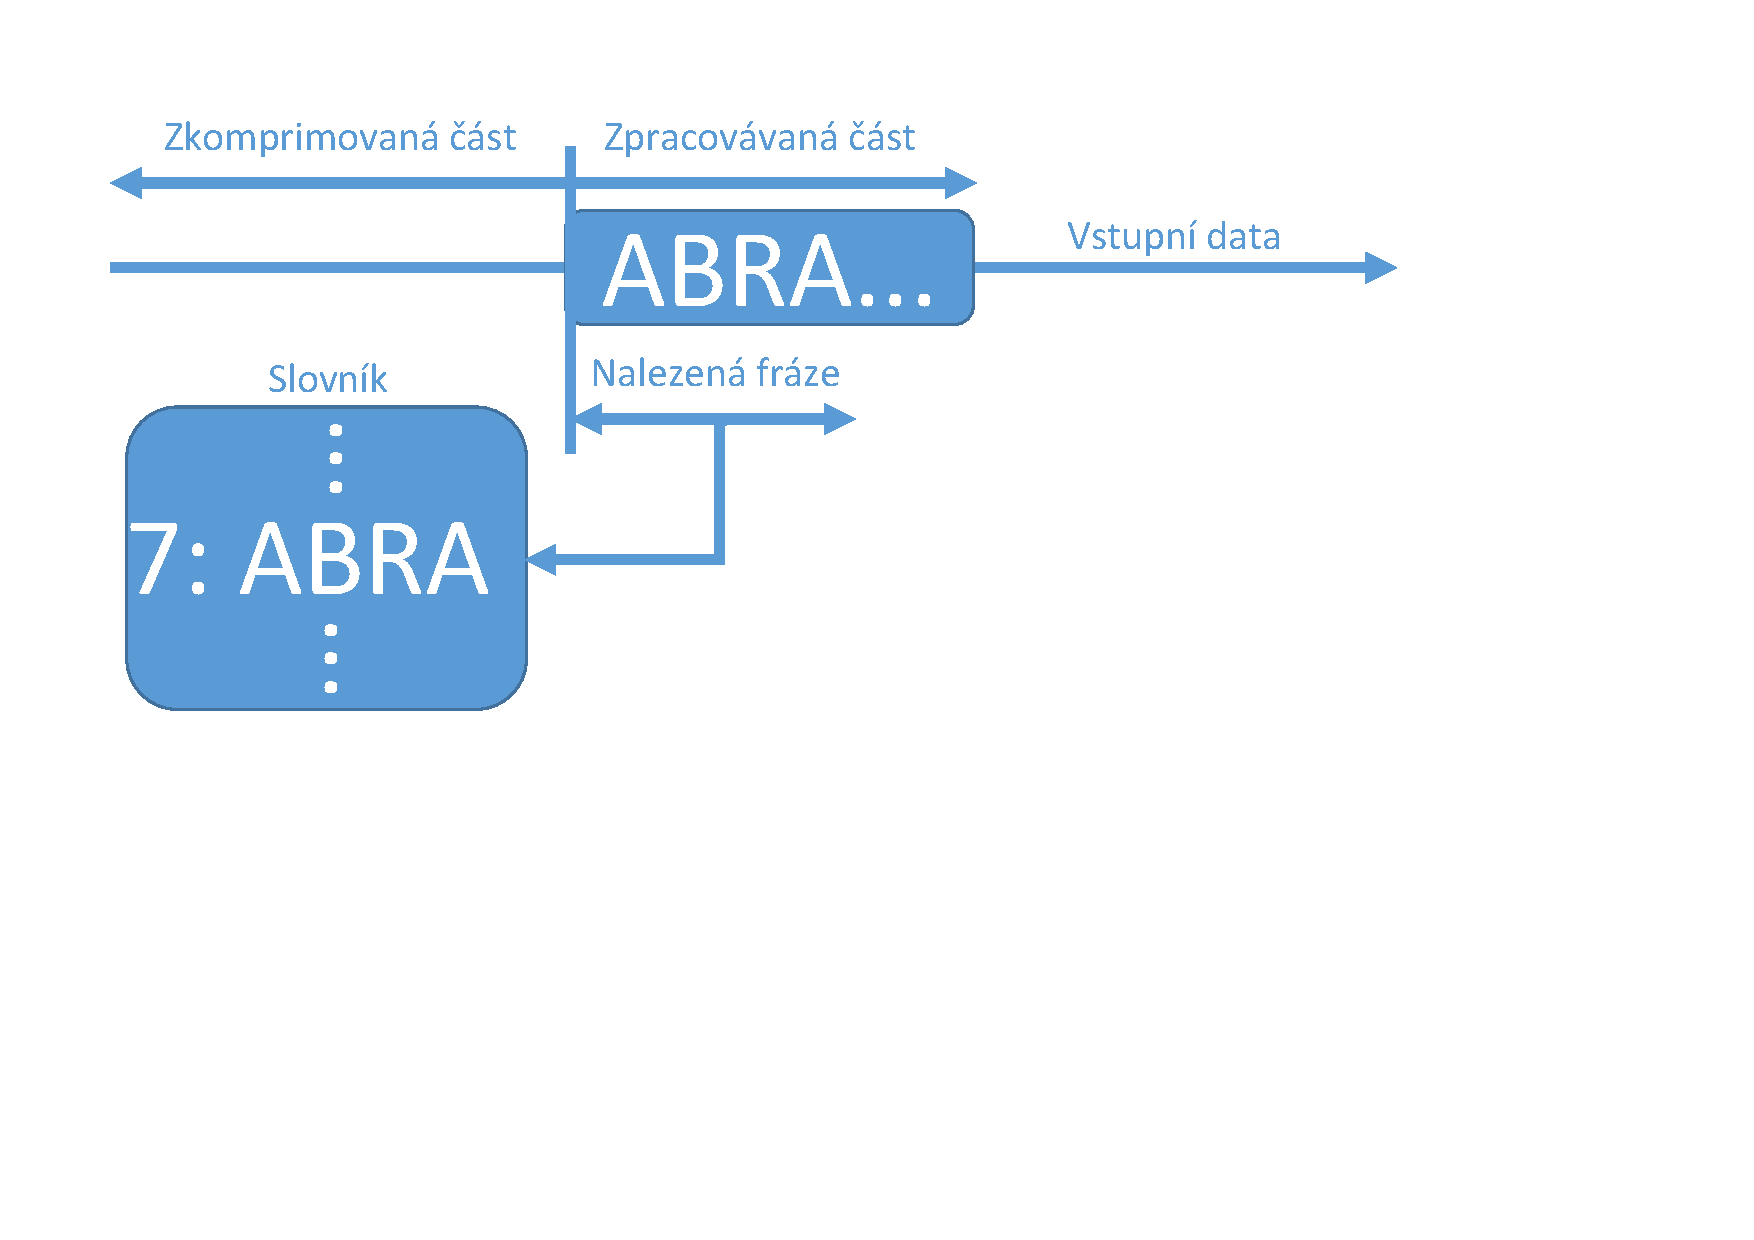
\includegraphics[trim=50 220 170 50, clip, angle=0, width=150mm]{slovnikLZ78}
\caption{Schéma algoritmu LZ78, jenž využívá vlastní slovník}
\label{slovnikLZ78}
\end{figure}

Vhodnou paměťovou strukturou pro uchovávání slovníku je strom, jehož uzly mohly mít tolik potomků, kolik je znaků zdrojové abecedy. V kořeni je prázdné slovo a při vyhledávání fráze se každým načteným znakem posuneme do potomka v příslušné větvi (pokud existuje).

\subsection{Princip komprese}
Na počátku je ve slovníku na pozici 0 pouze prázdné slovo\footnote{Prázdná posloupnost znaků, slovo délky 0.} $\varepsilon$. Při zpracování dat jsou na další pozice 1, 2 atd. vkládány nové fráze. Je-li na vstupu přečten znak $s$, algoritmus se ve slovníku pokusí nalézt jednoznakovou frázi $s$. Pokud není tato fráze nalezena, je vložena na volnou pozici s nejnižším indexem a na výstup je zapsána dvojice $(0,s)$, kde 0 je index prázdného slova. Tato dvojice znamená zakódování řetězce $\varepsilon s$ (zřetězení prázdného slova a znaku $s$). Naopak je-li fráze $s$ ve slovníku nalezena, je ze vstupu přečten další znak $t$ a ve slovníku je hledána dvouznaková fráze $st$. Pokud je fráze nalezena, pokračuje načítání dalších znaků a hledání ve slovníku. Pokud fráze nalezena není, je na výstup zapsána dvojice $(i,t)$, kde $i$ je index prefixové fráze $s$. Tento proces pokračuje, dokud nejsou zpracována všechna data na vstupu.

\subsection{Příklad komprese}
Zkusme pro příklad zakódovat část textu začínající slovem ABRAKADABRAK. Stav slovníku a výstup po kompresi můžeme vidět v tabulce \ref{LZ78tabulka}. V prvních třech krocích (indexy 1, 2 a 3) jsou komprimovány pouze jednoznakové fráze, v dalších krocích již existují fráze A, resp. AB a tedy jich můžeme využít k zakódování delších frází.

\begin{table}[!htb]
\catcode`\-=12
\centering
\begin{tabular}{|c|c|c|}
\hline
\multicolumn{2}{|c|}{Slovník} & \multirow{2}{*}{Výstup}\\
\cline{1-2}
Index & Fráze & \\
\hline
0 & $\varepsilon$ & \\
1 & $\mathrm{A}$ & $(0,\mathrm{A})$\\
2 & $\mathrm{B}$ & $(0,\mathrm{B})$\\
3 & $\mathrm{R}$ & $(0,\mathrm{R})$\\
4 & $\mathrm{AB}$ & $(1,\mathrm{B})$\\
5 & $\mathrm{ABR}$ & $(4,\mathrm{R})$\\
6 & $\mathrm{AK}$ & $(1,\mathrm{K})$\\
\hline
\end{tabular}
\caption{Kódování textu pomocí algoritmu LZ78}
\label{LZ78tabulka}
\end{table}

\subsection{Princip dekomprese}
Při rekonstrukci dat jsou čteny jednotlivé dvojice (index, znak) a slovník je vytvářen pomocí úplně stejných kroků jako v případě komprese. Je tedy složitější než dekompresní algoritmus LZ77. Plátí, že je-li nějaká fráze ve slovníku, pak jsou v něm i všechny její prefixy. Ty jsou nutné pro hledání delších frází, neboť kompresní algoritmus se odkazuje na prefixové fráze o jeden znak kratší.

\subsection{Variace algoritmu LZ78}
Podobně jako v případě algoritmu LZ77 vniklo i množství variant postavených na myšlence algoritmu LZ78 upravujících ty části, které považují autoři za neefektivní. Mezi nej\-vý\-zna\-mně\-jší se řadí metoda LZW vycházející z předpokladu, že kódovat jednotlivé znaky pomocí výše zmíněných dvojic je neefektivní. Místo toho na počátku kompresního procesu inicializuje slovník všemi jednoznakovými frázemi znaků zdrojové abecedy. Je-li hledaná fráze nalezena, pokračuje načtením dalšího znaku a hledáním delší fráze. Naopak, není-li fráze nalezena, je vložena do slovníku, ale na výstup kóduje pouze index o jeden znak kratší fráze nalezené ve slovníku (nalezení jednoznakové fráze je zaručeno díky původní inicializaci slovníku). Další hledaná fráze začíná posledním zpracovaným znakem, tj. posledním znakem fráze uložené do slovníku v předchozím kroku.